\documentclass[conference]{IEEEtran}
\IEEEoverridecommandlockouts
% The preceding line is only needed to identify funding in the first footnote. If that is unneeded, please comment it out.
\usepackage{cite}
\usepackage{amsmath,amssymb,amsfonts}
\usepackage{algorithmic}
\usepackage{graphicx}
\usepackage{textcomp}
\usepackage{xcolor}
\def\BibTeX{{\rm B\kern-.05em{\sc i\kern-.025em b}\kern-.08em
    T\kern-.1667em\lower.7ex\hbox{E}\kern-.125emX}}
\begin{document}

\title{Equilivest: A Robotic Vest to aid in Post-Stroke Dynamic Balance Rehabilitation
}

\author{%
Franco Paviotti$^{1}$, Esteban Buniak$^{2}$, Rodrigo Ramele$^{3}$, Orestes Freixes$^{4}$ and Juan Miguel Santos$^{5}$% <-this % stops a space
\thanks{$^{1}$F. Paviotti is with Bioengineering, Instituto Tecnológico de Buenos Aires
                    Buenos Aires, Argentina
        {\tt\small fpaviotti@itba.edu.ar}}%
\thanks{$^{2}$E.Buniak is with Ingeniería en Informática, Instituto Tecnológico de Buenos Aires
                    Buenos Aires, Argentina
        {\tt\small ebuniak@itba.edu.ar}}%
\thanks{$^{3}$R.Ramele is with Ingeniería en Informática, Instituto Tecnológico de Buenos Aires
                    Buenos Aires, Argentina
        {\tt\small rramele@itba.edu.ar}}%
\thanks{$^{4}$O. Freixes is with the CINER Centro Integral de Neurorehabilitación,
                    Buenos Aires, Argentina
        {\tt\small orestesfreixes@gmail.com}}%
\thanks{$^{5}$J.M. Santos is with the UNAHUR Universidad Nacional de Hurlingham,
                    Buenos Aires, Argentina
        {\tt\small juanmiguelsantos@gmail.com}}%
%\thanks{*This work was not supported by any organization}% <-this % stops a space}
}

%\author{\IEEEauthorblockN{1\textsuperscript{st} Franco Paviotti}
%\IEEEauthorblockA{\textit{Bioingeniería} \\
%\textit{Instituto Tecnológico de Buenos Aires}\\
%Buenos Aires, Argentina \\
%fpaviotti@itba.edu.ar}
%\and
%\IEEEauthorblockN{2\textsuperscript{nd} Esteban Buniak}
%\IEEEauthorblockA{\textit{Ingeniería en Informática} \\
%\textit{Instituto Tecnológico de Buenos Aires}\\
%Buenos Aires, Argentina \\
%ebuniak@itba.edu.ar}
%\and
%\IEEEauthorblockN{3\textsuperscript{rd} Rodrigo Ramele}
%\IEEEauthorblockA{\textit{Ingeniería en Informática} \\
%\textit{Instituto Tecnológico de Buenos Aires}\\
%Buenos Aires, Argentina \\
%rramele@itba.edu.ar}
%\and
%\IEEEauthorblockN{4\textsuperscript{th} Juan Miguel Santos}
%\IEEEauthorblockN{\textit{Ingeniería en Informática} \\
%\textit{UNAHUR}\\
%Hurlingham, Argentina \\
%jsantos@gmail.com}
%\and
%\IEEEauthorblockN{5\textsuperscript{th} Orestes Freixes}
%\IEEEauthorblockN{\textit{CINER} \\
%\textit{Centro Integral de NeuroRehabilitación}\\
%Buenos Aires, Argentina \\
%orestesfreixes@gmail.com}
%}

\maketitle

%\begin{abstract}
%Stroke is a medical condition that can affect motor function, particularly dynamic balance.  Biofeedback can aid in rehabilitaiton procedures which help patients to regain lost motor activity and recover functionality.  In this work, we are presenting a smart-vest device that assist in rehabilitation procedures by providing feedback in the form of vibrotactile stimulation. Information provided by principal caregivers, family, patient in the form of surveys and interview, is used to derive potential clinical causal hypothesis and these are used to drive the experimentation paradigm, and the robotic smart-vest to aid in the whole procedure...
%\end{abstract}

\begin{IEEEkeywords}
Stroke, Balance, Rehabilitation, Biofeedback, Vibrotactile
\end{IEEEkeywords}

\section{Introduction}

Brain stroke is a devastating medical condition, that affects world population and is the main cause of disabilities worldwide~\cite{Caplan.etal2023}.  Disabilities related to stroke can affect motor pathways, and may lead to several motor function disorders.   One important aspect of motor function is balance which is the ability to control the body's center of mass inside the base support provided by the lower limb~\cite{Bowman2021}.  Stroke can affect dynamic balance as well,  which is manifested while walking, impairing autonomy and independence, important factors in Activities of Daily Living (ADL) particularly for young patients~\cite{Afrasiabifar.etal2020,Donato.etal2016}.

% As early as possible the rehabilitation can be put into place, better the outcome that can be obtained by the treatment. 

Strong evidence suggests that neuroplasticity can be enhanced by neural rehabilitation~\cite{DeAngelis.etal2021,Albert.etal2012}.  These procedures are aimed to relearn movements that can trigger new neural pathway generation which reroute, or even completely replace, those pathways that were damaged by the stroke.   Recently, biofeedback techniques aiming to provide extra information to the patient to aid in the relearning, have appeared as a complementary treatment to increase neuralplasticity. These are in the form of Wearable devices-based biofeedback rehabilitation (WDBR)~\cite{Peake.etal2018} or robotic rehabilitation gait devices~\cite{Zhao.etal2022,Peshkin.etal2005,Tong.etal2006}.  

%Neurorehabilitation procedures are performed by a group of interdisciplinary caregivers and technicians. 

%This published evidence emphasizes that this biofeedback can indeed enhance the results of rehabilitation procedures.

Therefore, the addition of an independent and new peripheral therapeutic signal, that can be assimilated as an extrasensory input~\cite{Brandebusemeyer.etal2021},  could improve dynamic balance performance on post-stroke patients which may have yet insufficiency to deal properly with the complexities of walking.  Meaningful balance information, in terms of timing and location, can provide this extra signal in any form of stimulation, particularly vibrotactile feedback (VF).  Although the effectiveness of biofeedback on static balance has been studied more extensively in the literature~\cite{DeAngelis.etal2021}, to the best of our knowledge works dealing with dynamic balance problems while walking have been more scarce.

This work presents the development of a device which is grounded on this idea, and aims to help a post-stroke patient with a remaining dynamic balance problem, presenting it as a case study.  The proposed development is implemented as a smart-vest~\cite{Brandebusemeyer.etal2021}, which we will call, \textit{Equilivest}, that address three possible clinical hypothesis of the underlying problem.  We aim to provide motor learning, meaning to generate a fading compliant assist-as-needed vibrotactile feedback signal which is manifested to the patient as less conscious as possible~\cite{Srivastava.etal2016,Donato.etal2016}.  The device aims to promote plasticity by producing timing vibrotactile stimulation based on kinematic and dynamics measurements.  

%The idea is to exploits these ideas from neurofeedback that we can create "external" sensors by providing some form of vibrotactile stimulation on her belly and link that stimulation to some form of measurements from IMUs (inertial sensors).

%The form of validation procedures that is required in clinical settings\cite{Papastylianou.etal2016}.

%Section \ref{sec:case-study} presents the case study.  Next section \ref{sec:hypothesis} summarize the results of the interviews and surveys performed by the patient, their family and professional caregivers, presenting the underlying clinical causal hypothesis.  Section \ref{sec:vest} describes the vest details and architecture.  The experimental design protocol is expounded in Section \ref{sec:experimental}.  Preliminary results are presented on the next section, and this work concludes with discussion and conclusion.

\section{Materials and Methods}

\subsection{Patient Case Study}
\label{sec:case-study}

Patient is a 31 years old female, without any history of chronic ailment, who suffered an acute brainstem stroke after giving birth.  The stroke was on posterior fossa subarachnoid due to a brain artereovenous malformation (AVM), which could be linked to pregnancy or puerperium~\cite{Porras.etal2017}.  Patient was in coma for around 2 months, and after that unable to walk, move, talk or swallow.  After two years of intensive rehabilitation, Patient managed to recover significantly, including from dysphagia, which was very important in order to remove the feeding tube allowing her to start speech recovering.  

After 24 months since event, the patient, was discharged from hospital and maintained a 3 times per week rehabilitation treatment, focusing on a remaining affection related to dynamic balance problems while walking.  The patient achieved satisfactory index scores in static balance tests and is able to perform static hip-balance and ankle-balance.  She has recovered muscle in her legs and can perform lower-limb exercises.  Her vision is normal.   

However, when the patient tries to walk on open-spaces, or with confronting lights (like walking towards sunlight), with other people moving around, or when concentration fades while walking, she is unable to keep up with the pace of the gait and the risk of fall increases.  Nowadays, the patient walks freely unaided at home but requires a Canadian cane otherwise.

%\begin{table*}[t]
%\begin{center}
%\begin{tabular}[!t]{|c|c|}
%\hline
%Question & Avg. answer \\
%\hline
%Podes describir cómo y cuándo se expresa la perdida del equilibrio y su proceso? - Esta pregunta nos servirá para determinar con mayor precisión los métodos de sensado y alarma a desarrollar  & Cuando estoy cansada, distraída o muy nerviosa\\
%\hline
%¿Siempre se desarrolla de la misma manera? - Con esta pregunta queremos profundizar sobre la anterior con el objetivo de una mejor comprensión &  Si \\
%\hline
%¿Cuál? Si la respuesta fue no, deje sin contestar  & Me desequilibro\\
%\hline
%¿Podés evidenciar cuando estas por empezar a perder el equilibrio? - Con esta pregunta intentamos conocer un fenómeno que permita detectar el principio de caída & Si \\
%\hline
%Si la respuesta fue si ¿Qué sentís? & Un poco no siempre siento inestabilidad previo  \\
%\hline
%¿Con qué frecuencia usas el andador? - Puede seleccionar mas de una opción. Así nos ayudará a entender mejor el cuadro & Solo fuera de casa \\
%\hline
%¿Existe algún denominador común en las caídas? - La presencia de este sería importantísima para  un fenómeno o señal a medir y caracterizar que sería muy útil para la detección del principio de caídas. Si hay algo que siempre se repite podríamos enfocarnos en detectar eso. & Si \\
%\hline\\
%¿Cuál? Si la respuesta fue "No" deje la respuesta en blanco & Lo que anteriormente dije estoy cansada o distraída o nerviosa  \\
%\hline
%¿Cómo estás trabajando la recuperación hoy por hoy? - Con esta pregunta buscamos conocer el estado de situación y trabajo actual & Fortalecimiento de músculos   \\
%\hline
%¿Hay algo más que desees comentar o expresar? & No uso andador es un bastón canadiense. 
%Ahora me doy cuenta antes que me voy a caer, pero queda poco para evitarlo.   \\
%\hline
%\end{tabular}
%\caption{table}{Answers to survey questions.}
%\label{tab:alpi_q_table_1}
%\end{center}
%\end{table*}



%\begin{table*}[t]
%\begin{center}
%\begin{tabular}[!t]{|c|c|}
%\hline
%Question & Avg. answer \\
%\hline
%¿Cuál es la razón de la pérdida del equilibrio en la paciente? - Esta pregunta nos permite conocer la opinión de los profesionales e interiorizarnos en el caso.  & Lesión en el tronco del encéfalo\\
%\hline
%¿Podes describir cómo y cuándo se expresa la perdida del equilibrio y su proceso? - Con la descripción podemos comprender como y en que circunstancias se desencadena el fenómeno de la caída y conocer mejor el caso. &  La pérdida del equilibrio se expresa en el inicio y durante la marcha. cuando se detiene también. Camina con compensación visual y cuando quita la vista el suelo (ej mira para el costado aumenta la inestabilidad) Realiza una marcha sin el automatismo habitual. Le demanda mucha concentracion.  \\
%\hline
%¿ La paciente puede caminar sin un dispositivo de tipo ayuda marcha? De ser así, ¿Bajo que circunstancias? - Conociendo mejor la situación actual podemos tomar mejores decisiones en cuanto a como posicionar sensores y medir.  & Solo de manera  terapéutica. habitualmente la trabajamos con máxima supervisión.\\
%\hline
%¿Presenta una pérdida de fuerza muscular que dificulte el caminar? - Esta pregunta permite conocer el caso en mayor detalle  con propiedad para evitar adelantarnos a hipótesis de trabajo erróneas. & No \\
%\hline
%¿Presenta dismetría? - Nuevamente queremos adelantarnos a hipótesis erróneas a la hora de decidir el método de sensado y procesamiento de las señales. La longitud o duración de los movimientos puede usarse como un indicador para nosotros, como también asi los ritmos. & Si \\
%\hline
%¿Presenta temblores?  - En caso de presentar temblores estos se verán reflejados en las señales y es útil tenerlo en cuenta ya que caracterizará a nuestra señal. & No \\
%\hline
%¿Presenta alteraciones en la marcha en instantes previos a la caída? - En caso de existir algún impulso inicial que podamos sensar o medir de forma indirecta podemos anticiparnos a la perdida del equilibrio en las señales. & Si \\
%\hline\\
%¿Cuáles? Si la respuesta fue "No" deje en blanco & Fallas las reacciones de tobillo y cadera \\
%\hline
%¿Sufrió alteraciones en la sensibilidad profunda? - Existe un trabajo previo en la Universidad de Buenos Aires que usa un método de sensado orientado a la presión de la pisada. Esto puede orientarnos en otro sentido en el sensado y estimulación. & No  \\
%\hline
%Antes de perder el equilibrio, ¿Trastabilla?¿Acelera la marcha? -  Al igual que en otras preguntas buscamos obtener información extra para el  procesamiento de las señales y detección del principio de caída. Estos fenómenos pueden medirse o detectarse y evidenciarían el inicio de una posible caída. & Otro síntoma  \\
%\hline
%Si la respuesta fue 'Otro síntoma' ¿Cuál? - En caso contrario deje sin responder & Reacción lenta \\
%\hline
%¿Presenta algún tipo de marcha patológica? -la caracterización del caso permite decidir formas y métodos de sensado y procesamiento. & Si  \\
%\hline
%¿Cuál? Si la respuesta fue "No" deje la respuesta en blanco & Marcha Atáxica \\
%\hline
%¿Existe algún denominador común en las caídas? - La presencia de este sería importantisima para  un fenómeno o señal a medir y caracterizar que sería muy útil para la detección del principio de caídas. Si hay algo que siempre se repite podríamos enfocarnos en detectar eso. & Si \\
%\hline
%¿Cuál? Si la respuesta fue "No" deje la respuesta en blanco & El denominador es cuando deja de realizar la marcha de manera consciente. Por ejemplo, cuando camina y tiene que realizar alguna tarea que implique procesos cognitivo. Dual Task  \\
%\hline
%¿Se hizo un estudio de evaluación de marcha? - Esta pregunta podría aportar información suplementaria a preguntas anteriores que nos permiten conocer e interiorizarnos en el caso & No  \\
%\hline
%¿Se hizo evaluación de riesgo de caídas? - Esta pregunta puede aportar algo de información extra para el conocimiento del caso. & Si  \\
%\hline
%¿Hay alguna manera en que trabaje en la reeducación de la paciente? -  Quisiéramos conocer un poco mas la situación actual y las actividades que realiza la paciente para su recuperación. & Si a través de la reeducación del VOR,  facilitación del equilibrio estático y dinámico, entrenamiento del automatismo de la marcha con diferentes niveles de dificultad.  \\
%\hline
%¿Hay algo mas que desee comentar o expresar?  & Mes a mes se evidencia una mejora, todavía no alcanza para que pueda caminar sin supervisión.  \\
%\hline
%\end{tabular}
%\caption{table}{Answers to survey questions.}
%\label{tab:alpi_q_table_1}
%\end{center}
%\end{table*}


\subsection{Underlying hypothesis}
\label{sec:hypothesis}

Human balance is composed of a complex interaction of different subsystems, which includes somatosensorial information, vestibular system and visual information as input sources.  These are later processed in different networks of the Central Nervous System (CNS), and finally actuated by motor pathways at many different scales~\cite{Donato.etal2016}.

\begin{table*}[t]
\begin{center}
\begin{tabular}[!t]{|p{0.45\linewidth} |p{0.45\linewidth} |}
\hline
\textbf{Question} & \textbf{Answer} \\
\hline
\hline
Under which situations do you feel you are prone to fall ? & When I am tired, distracted or stressed. \\
\hline
What do you feel ?  & I feel that I loss my balance\\
\hline
What do you feel before you fall ? & Sometimes I do feel something before.  I realize that I am going to fall, but there isn't anything I can do to avoid it. \\
\hline
When do you use the cane ?  & Only when I am out of home.\\
\hline
\end{tabular}
\vspace{2pt}
\caption{Survey and responses provided by the patient and family.}
\label{tab:patientsurvey}
\end{center}
\end{table*}

\begin{table*}[t]
\begin{center}
\begin{tabular}[!t]{|p{0.45\linewidth} |p{0.45\linewidth} |}
\hline
\textbf{Question} &  \textbf{Answer} \\
\hline
\hline
Describe the situation when the patient loss her balance & Loss of balance is manifested at the beginning, during the gait cycle or with sudden stops. Walking is performed using intense visual compensation.   Instability increase when the patient is distracted, when she stops looking at the floor, or when she looks sideways.  Her gait is not automated, and demands cognitive resources. \\
\hline
Is there any significant muscle loss in lower-limbs ? & No\\
\hline
Does she presents any of the following dysmetria / heavy shaking / somatosensorial alterations / proprioceptive alterations ? & No \\
\hline
Does she have any visible reaction before falling?  & She presents dynamic alterations in hip and ankle compensation.\\
\hline
Is the patient gait normal ?  &  No, the patient presents ataxic gait, likely triggered by slow reaction to perform lower-limb balance correction. \\
\hline
Is there any behavioral pattern linked to falling events ? &  Yes, cognitive workload.  Dual tasks situations, when the patient needs to perform something extra while walking. \\
\hline
Describe current treatment. & The patient is currently working on rehabilitation exercises to retrain her Vestibulo-Ocular Reflex (VOR), to improve her static and dynamic balance, and improve her locomotor automatism.  She is improving on a monthly basis, but still she has not reached the level to walk autonomy without any aid. \\
\hline
\end{tabular}
\vspace{2pt}
\caption{Survey and responses provided by his main patient's rehabilitation caregiver.}
\label{tab:caregiverssurvey}
\end{center}
\end{table*}

We perform a series of surveys and interviews with the patient and their caregivers.  Main results are summarized in 
Tables ~\ref{tab:patientsurvey} and \ref{tab:caregiverssurvey}.  Based on the clinical history, results from surveys and interviews, we postulate three different potential clinical situations that could use the external biofeedback signal and could potentially aid in rehabilitation procedures.  The first (i) is a potential problem in the integration of vestibular information while walking, the second (ii) is bradykinesia where the required processing speed to effectively adjust the lower limb to keep the center of mass inside the base support is not achieved.  Finally, the third (iii) hypothesis is an ataxic gait, where non-automated gait produces an increase in the likelihood of failing.

%Bradykinesia: due to the slow speech.
%Unusual gait
%Dysmetria (visual?) (ataxia?)

%\begin{itemize}
%\item Vestibular information or fusion of vestibular information
%\item Bradykinesia: the processing speed required to effectively perform the processing and actuation is not enough.
%\item Ataxic gait: the movement is not normally regulated.
%\end{itemize}
%

\subsection{Robotic Device Vest}
\label{sec:vest}

The vest system prototype is based on Internet of Robot Thing (IoRT) technology~\cite{Simoens.etal2018,Domingo.etal2012}. The controller is an Arduino UNO (Arduino LLC, Italy) board coupled with ESP8266 shield (WeMos, United Kingdom).  The system is powered by a commercial power bank with Li-Po 18650 cells (Ipower, United States). It also contains an Inertial Measurement Unit (IMU) MPU 6050 (OEM ITG/MPU6050) and a FA-12350 DC motor scavenged from old compact discs which provide the vibrotactile feedback.  The IMU provides accelerometer and gyroscope data to get a 3-dimensional angular acceleration vector and a linear acceleration vector. Pitch, Roll and Yaw angles are calculated from a set of transforming equations and processed with a complementary filter which relies $0.98$ in gyroscope data and $0.02$ in accelerometer data~\cite{Fetick.2022}. These values are transmitted by telemetry in real-time as UDP packets for off-board register, processing and further analysis. Data recovered by the device is sampled at 100 Hz. The smart-vest prototype can be seen in Figure~\ref{fig:smart-vest}.  It is based on a safety vest, complemented with Velcro pockets. 

\begin{figure}[h!]
\centering
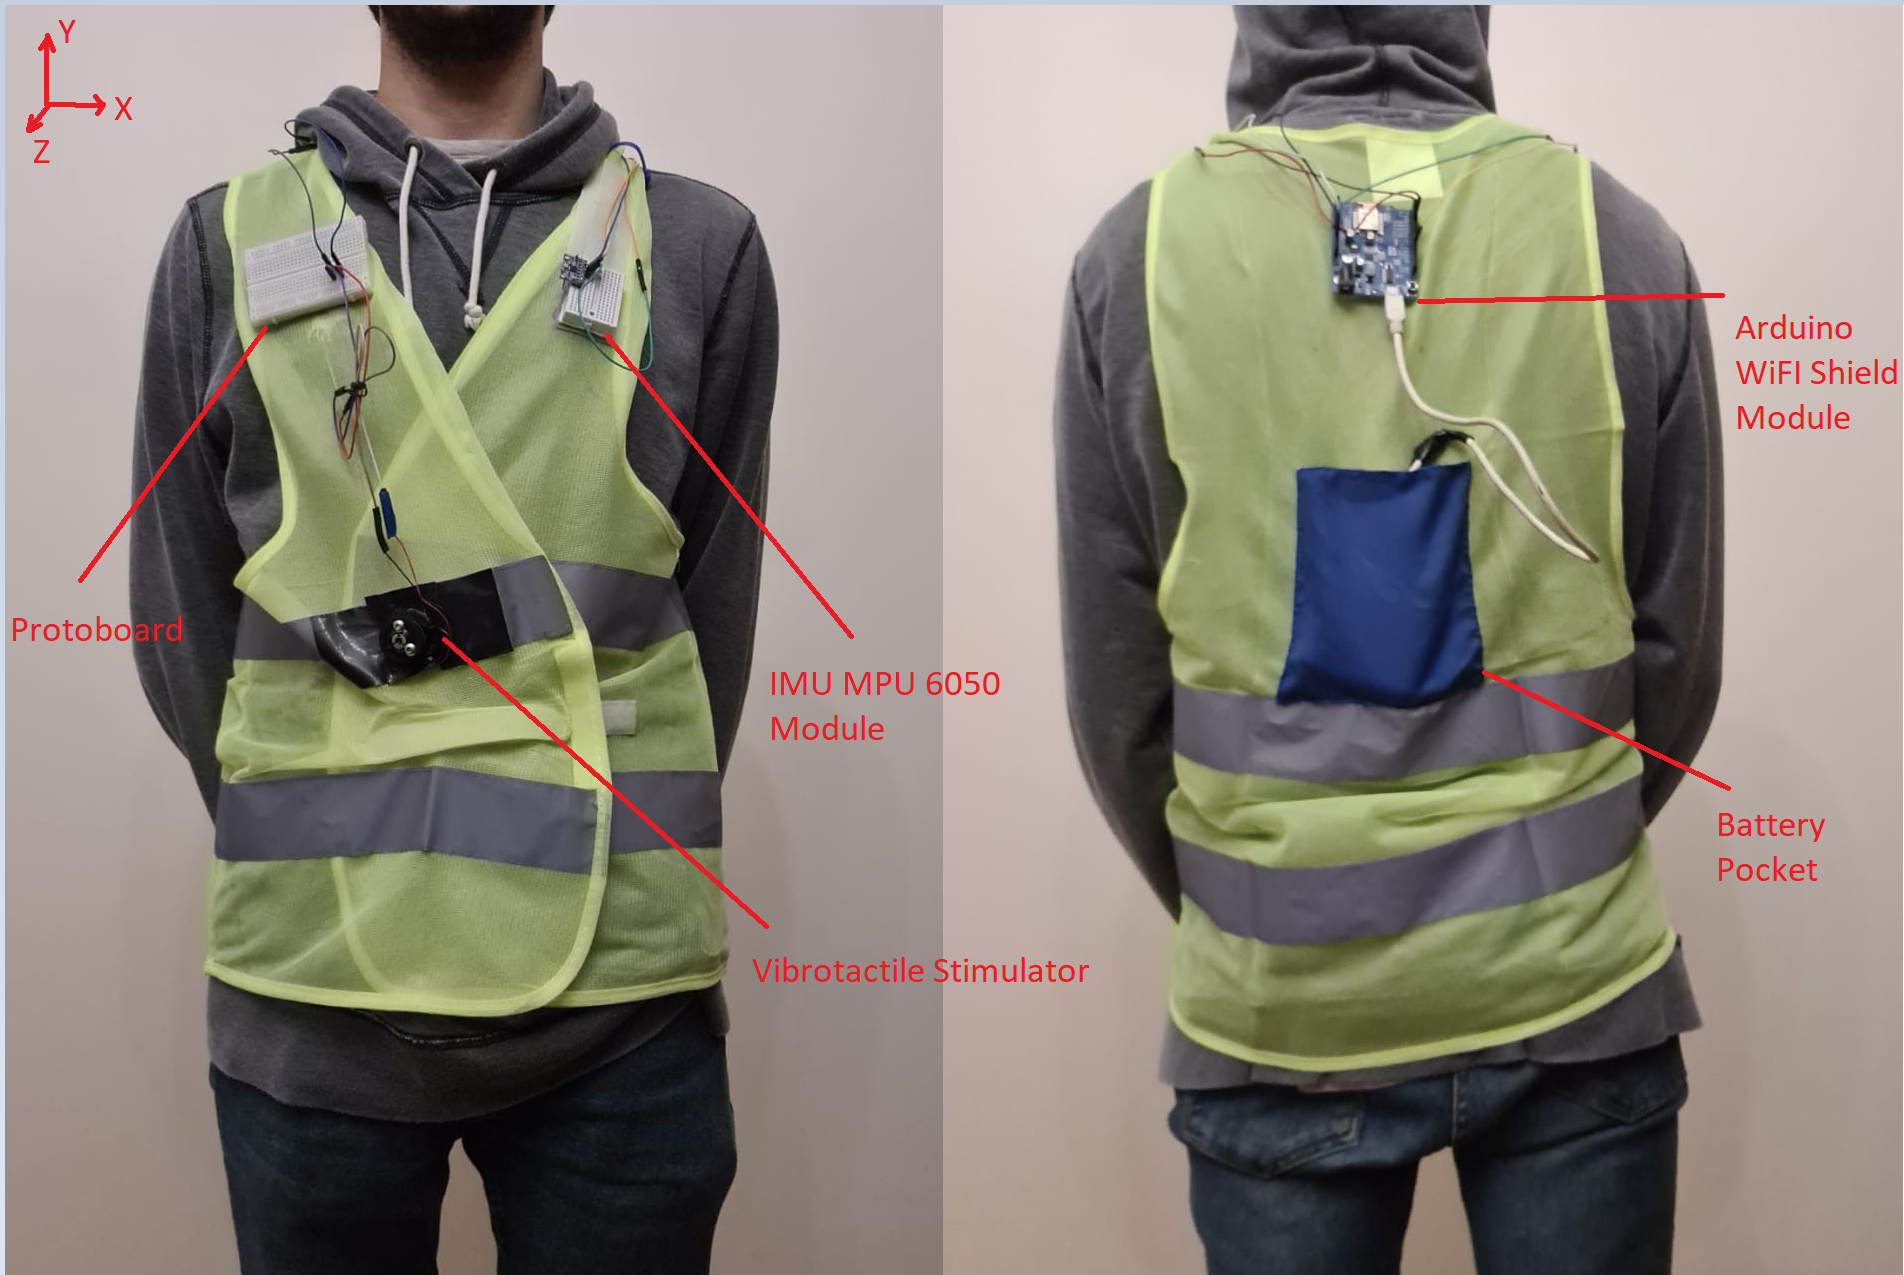
\includegraphics[width=8cm]{equilivest.png}
\caption{Front and back view of the Equilivest prototype.  The vest is based on a safety vest, with additional velcro pockets.  The battery is located on the back, while the vibrotactile motor is located on the belly~\cite{Brandebusemeyer.etal2021}.  The IMU sensor is pressed against the chest by the use of a flexible elastic band. }
\label{fig:smart-vest}
\end{figure}




%\textbf{Why only vibrotactile stimulation and not auditory stimulation}

\subsection{Experimental Design}
\label{sec:experimental}

Three experiments are designed in order to assess each one of the potential clinical causes, and to derive for each one of them a stimulation strategy.  Participants are recruited voluntarily and the experiment is conducted anonymously in accordance with the declaration of Helsinki published by the World Health Organization. No monetary compensation is handed out and all participants agree and sign a written informed consent. This study is approved by the Departamento de Investigación y Doctorado, Instituto Tecnológico de Buenos Aires (ITBA).  All the participants wear the smart-vest with an elastic band pressed tightly towards the chest, tied in no-restrictive manner, holding the sensor firmly. 

%\begin{itemize}
%\item Controlamos que la posición del IMU no supere un umbral, y si lo hace vibra el motor.
%\item Intentamos predecir una situación de caída y generar un alerta antes de que ocurra.
%\item Hacemos un pacemaker.  Es decir una estimulación sincrónica asociada a la detección de un podómetro.
%\end{itemize}

\subsubsection{Vestibular Information Integration}

This experiment aims to study the falling process. Participants are told to lean forward until they couldn't maintain balance anymore and let themselves fall into a mattress. This experiment is used to determine a threshold for the data that can help to identify the breakpoint conditions based on the IMU information where each subject falls.

In order to test it, 5 healthy participants are recruited to perform 10 runs of falling situations  Participants wearing the vest  perform a one-step forward walking exercise with the upper-trunk leaned forward at different angles progressively until they can no longer cope with the unbalance situation and fall to the mattress.

\subsubsection{Ataxic Gait}

This experiment has the purpose of analyzing and studying gait's behavior. In order to accomplish this,  5 participants are instructed to perform 10 sessions of walking in a straight line across ten meters, performing Ten-Meter Walking (10MWT) assesment~\cite{Olmos.etal2008}.  We collected and analyzed pitch, roll and yaw values as well as angular acceleration changes registered by the IMU gyroscope. In this study our goal is to be able to process and identify gait abnormalities as well as all steps occurring and any fall that might develop. 



\subsubsection{Bradykinesia}

This experiment involves the coupling of the other two.  Five participants are instructed to perform 10 runs of a ten-meter walking procedure, followed by a falling into a mattress.  The purpose of this experiment is obtain a multichannel time series of the whole sequence, including the walk and the falling action.

%(3) Ver en base a la encuesta como se da la situación de caída más común que Paula relata, en base a lo que ella manifiesta.  Entonces lo que hacemos es tomamos 5 sujetos y los hacemos caer 5 veces cada uno sobre la colchoneta (o 10 o 20 x sujeto, lo que más puedas).  Con estos datos, que son series de tiempo de 6 variables, intetamos ver si con un modelo de ML podemos predecir el momento de la caída simulada de cada uno de ellos y ANTICIPARNOS .  La idea entonces es que suene el motor cuando el sistema detecta con antelación que puede venir una caída inminente.  Aca se muestra el accuracy en la detección de la caída en los datos recabados.

%(4) En este caso, lo que hacemos es armar un gráfico de gait y lo que hace el dispositivo es detectar un punto en el ciclo y vibrar de forma recurrente, como un marca paso, basado en un podómetro.  En este caso, tomás 5 personas las hacés caminar, determinás cómo son esas curvas y accionás el motor siempre en el mismo momento.  Lo que mostramos son los gráficos y el momento donde se dispara la estimulación.


\section*{Results and Discussion}

Preliminary results show that for the (1) experiment (Figure \ref{fig:vestibular}), the pitch,roll, yaw angles can be used to determine a breakpoint where the fall is inevitable (black vertical line, marked as 1).   Results from experiment number (2) in Figure \ref{fig:gait} show that the gait cycle are clearly visible from raw acceleration data.

\begin{figure}[h!]
\centering
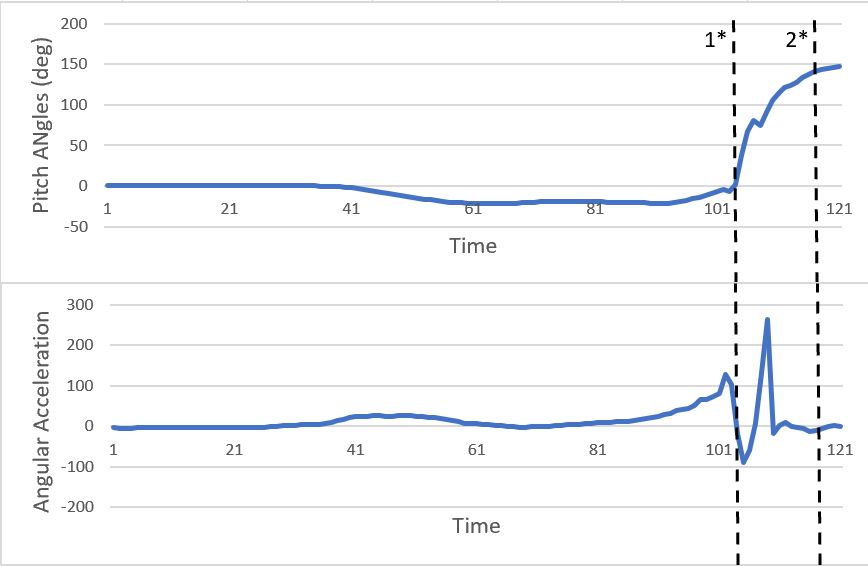
\includegraphics[width=8cm]{vestibular.png}
\caption{Pitch value in degrees showing the progressive increase as participants leaned forward crossing the instability condition (1).  Time is in milliseconds. }
\label{fig:vestibular}
\end{figure}


\begin{figure}[h!]
\centering
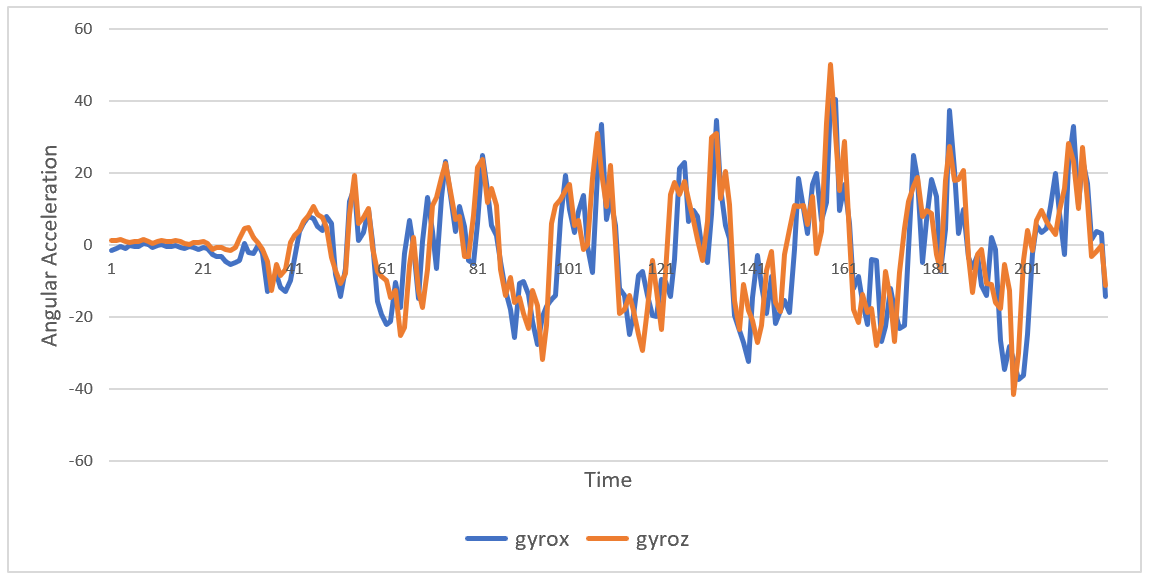
\includegraphics[width=8cm]{gait.png}
\caption{Angular acceleration for the X and Y axis showing 7 steps of the 10MWT assessment.  Time is in milliseconds. }
\label{fig:gait}
\end{figure}

%(1) Se muestran entonces esos dos gráficos promediados de cada uno de los 5 sujetos (10 series, 5 sin el motor, 5 con el motor).
%
%
%(2) Se muestra los gráficos de las series de tiempo offline de los datos analizados y como el sistema online de predicción acierta justamente en anticipar la caída.  (Esto es probablmente desde software lo más complejo).
%
%(3) Este caso probablemente sea el que requiera más experimentación sobre Paula en sí misma.  La idea acá es tener los gráficos promediados de GAIT, que son todos cíclicos, de dos de las variables cualquiera del IMU que formen un ciclo, y ver que hay un patrón común que se da más o menos para las personas healthy.  En base a eso, luego la idea es probar si con Paula ese patrón CAMBIA.  A partir de que vemos si cambia hay que ver donde cambia y en ese punto meter el pacemaker.


The information provided from all the experiments allow us to implement three different VF strategies:  The first is an \textbf{Artificial Vestibular Feedback}, which provides information as a feedback for vestibular information integration process.  This is implemented as a frequency-increasing VF signal that represents a distance from the breaking condition position where the fall is inevitable.   The purpose is to provide the patient with a continuous sensation that modulates the risk of falling.

The second strategy is the implementation of \textbf{Gait Pacemaker}.  The obtained data from the analysis of the ataxic gait is used to implement a podometer.  It has been showed that gait synchronization with music increase gait performance~\cite{Roerdink.etal2007} and synchronized gait trainer achieved positive results on patient~\cite{Blicher.etal2009}.  Hence, the aim of this stimulation approach is to keep the patient as close as possible to a normal and safe gait.

The final stimulation scheme deals with the Bradykinesia condition, and aims to have a \textbf{Risk-Predictor}~\cite{Rahman.etal2022,Ali.etal2022}.  The IMU data  represents a multichannel time series.  Hence, it can be used to predict a risk of falling, ahead of its occurrence, by building a machine-learning predictor based on the analysis of the time-series data.  The rationale is to counter the slowness of the response by predicting the falling situation ahead of its occurrence and providing the VF stimulation to force a change in the risky gait pattern.

%Hence, the signals  IMU can be feed back to the patient by vibrotactile stimulation on their belly. This will be impemented, first, in a binary way.  The hypothesis is that if there is a vestibular problem that forbids the patient to receive or evaluate the vestibular information appropriately, this external signal can be available for the patient to integrate it into the dynamic balance system.

%Afterward, the experiment will be repeated with the 5 participants activating the vibrotactile stimulation which will map progressively the inclination angle.  Hence it will provide an extra signal that can give a accurate information in relation to the stability of the upper-trunk in relation to the walking gait.

\section*{Conclusion}
Overall, this devices allows to implement a testbed that can be iteratively extended to obtain experimental data and to implement biofeedback strategies which could potentially lead to an increase in the effectiveness of different rehabilitation procedures~\cite{Bowman2021}.


%\section*{Acknowledgment}

%The preferred spelling of the word ``acknowledgment'' in America is without 
%an ``e'' after the ``g''. Avoid the stilted expression ``one of us (R. B. 
%G.) thanks $\ldots$''. Instead, try ``R. B. G. thanks$\ldots$''. Put sponsor 
%acknowledgments in the unnumbered footnote on the first page.

%Please number citations consecutively within brackets \cite{b1}. The 
%sentence punctuation follows the bracket \cite{b2}. Refer simply to the reference 
%number, as in \cite{b3}---do not use ``Ref. \cite{b3}'' or ``reference \cite{b3}'' except at 
%the beginning of a sentence: ``Reference \cite{b3} was the first $\ldots$''
%
%Number footnotes separately in superscripts. Place the actual footnote at 
%the bottom of the column in which it was cited. Do not put footnotes in the 
%abstract or reference list. Use letters for table footnotes.
%
%Unless there are six authors or more give all authors' names; do not use 
%``et al.''. Papers that have not been published, even if they have been 
%submitted for publication, should be cited as ``unpublished'' \cite{b4}. Papers 
%that have been accepted for publication should be cited as ``in press'' \cite{b5}. 
%Capitalize only the first word in a paper title, except for proper nouns and 
%element symbols.
%
%For papers published in translation journals, please give the English 
%citation first, followed by the original foreign-language citation \cite{b6}.

\bibliographystyle{IEEEtran}
\bibliography{iros}


%
%\vspace{12pt}
%\color{red}
%IEEE conference templates contain guidance text for composing and formatting conference papers. Please ensure that all template text is removed from your conference paper prior to submission to the conference. Failure to remove the template text from your paper may result in your paper not being published.

\end{document}
